\documentclass{beamer}
\usepackage{listings}
\lstset{
%language=C,
frame=single, 
breaklines=true,
columns=fullflexible
}
\usepackage{subcaption}
\usepackage{url}
\usepackage{tikz}
\usepackage{tkz-euclide} % loads  TikZ and tkz-base
%\usetkzobj{all}
\usetikzlibrary{calc,math}
\usepackage{float}
\newcommand\norm[1]{\left\lVert#1\right\rVert}
\renewcommand{\vec}[1]{\mathbf{#1}}
\providecommand{\pr}[1]{\ensuremath{\Pr\left(#1\right)}}
\providecommand{\brak}[1]{\ensuremath{\left(#1\right)}}
\usepackage[export]{adjustbox}
\usepackage[utf8]{inputenc}
\usepackage{amsmath}
\usetheme{Boadilla}
\title{CHARACTERISTIC FUNCTIONS}
\author{ANANTHOJU PRANAV SAI - AI20BTECH11004}

\begin{document}
\begin{frame}
\titlepage
\end{frame}
\begin{frame}{Characteristic function}
The Characteristic function of random variable X is defined as
\begin{align}
    C_{X}(t)=\mathbb{E}[e^{itX}]
\end{align}
which can also be written as
\begin{align}
    C_{X}(t)=\int e^{itx} \,d\mathbb{P}_X
\end{align}
If X is a continuous random variable with density function f_{X}(x), then\\
\begin{align} 
    C_{X}(t)=\int e^{itx}f_{X}(x)\,dx
\end{align}
\end{frame}
\begin{frame}{Elementary properties of characteristic functions}
 \begin{itemize}
     \item If $Y=aX+b$ ,then $C_Y(t) =e^{ibt}C_X(at)$.
     \item If $X$ and $Y$ are independent random variables and $Z=X+Y$, then $C_Z(t) =C_X(t)C_Y(t)$
 \end{itemize}   
\end{frame}
\begin{frame}{Example Question}
\begin{block}{Question}
    Find the characteristic function of $Y=\sum_{r=1}^{n}a_rX_r$, where $a_1,a_2,...,a_n$ are constants and $X_1,X_2,X_3,..,X_n$ are random variables, each of which takes the values -1 and 1 with probability $\frac{1}{2}$. Taking $a_r=2^{-r}$ for each $r$, show that $Y$ converges in distribution to uniform distribution on (-1,1).
\end{block}
\end{frame}
\begin{frame}{Solution}
Given,
\begin{align}
    Y&=\sum_{r=1}^{n}a_rX_r
\end{align}
The characteristic function of a random variable Y is defined as
\begin{align}
    C_{Y}\brak{t}&=E[e^{itY}]\\
    \implies C_{Y}(t)&=E[e^{it\sum_{r=1}^{n}a_rX_r}]\\
    \implies C_{Y}(t)&=\prod_{r=1}^{n}E[e^{ita_rX_r}]\\
    \implies C_{Y}(t)&=\prod_{r=1}^{n}C_{X_r}(a_rt)
\end{align}
\end{frame}
\begin{frame}{Solution contd.}
By taking $a_r=2^{-r}$ we get,
\begin{align}
    C_{Y}\brak{t}&=\prod_{r=1}^{n}C_{X_r}\brak{\frac{t}{2^r}}
    \label{a}
\end{align}
As random variables $X_r's$ follow discrete uniform distribution with only two possible outcomes ($X_r=-1$ and $X_r=1$) the characteristic function of $X_r$ is
\begin{align}
    C_{X_r}\brak{t}&=\sum_{k}e^{ikt}\pr{X_r=k}\\
    \implies C_{X_r}\brak{t}&=\frac{e^{-it}}{2}+\frac{e^{it}}{2}\\
    \implies C_{X_r}\brak{t}&=\frac{1+e^{2it}}{2e^{it}}\\
    \implies C_{X_r}\brak{\frac{t}{2^r}}&=\frac{1+e^{2i\brak{\frac{t}{2^r}}}}{2e^{i\brak{\frac{t}{2^r}}}}
        \label{b}
\end{align}
\end{frame}
\begin{frame}{Solution contd.}
 using \eqref{b} in \eqref{a}
\begin{align}
    C_{Y}\brak{t}&=\prod_{r=1}^{n}\brak{\frac{1+e^{2i\brak{\frac{t}{2^r}}}}{2e^{i\brak{\frac{t}{2^r}}}}}\\
    \implies C_{Y}\brak{t}&=\frac{\brak{1+e^{it}}\brak{1+e^{i\brak{\frac{t}{2}}}}....\brak{1+e^{i\brak{\frac{t}{2^{n-1}}}}}}{2^n\brak{e^{i\sum_{r=1}^n\frac{t}{2^r}}}}\\
     \therefore C_{Y}\brak{t}&=\frac{\brak{e^{2it}-1}}{2^ne^{it\brak{\frac{2^{n+1}-1}{2^{n+1}}}}\brak{e^{\brak{\frac{it}{2^{n-1}}}}-1}}
     \label{c}
\end{align}   
\end{frame}
\begin{frame}{Solution contd.}
    Now consider
\begin{align}
     \lim_{n\to\infty} C_{Y}\brak{t}
     \label{d}
\end{align}
using \eqref{c} in \eqref{d}
\begin{align}
    \implies \lim_{n\to\infty}\frac{\brak{e^{2it}-1}}{2^ne^{it\brak{\frac{2^{n+1}-1}{2^{n+1}}}}\brak{e^{\brak{\frac{it}{2^{n-1}}}}-1}}
    \label{e}\\
    \implies \lim_{n\to\infty}\frac{\brak{e^{2it}-1}}{2ite^{it\brak{\frac{2^{n+1}-1}{2^{n+1}}}}\frac{\brak{e^{\brak{\frac{it}{2^{n-1}}}}-1}}{\brak{\frac{it}{2^{n-1}}}}}
    \label{e}
\end{align}
\end{frame}
\begin{frame}{Solution contd.}
    We know that,
\begin{align}
    \lim_{n\to\infty}e^{it\brak{\frac{2^{n+1}-1}{2^{n+1}}}}&=e^{it}
    \label{g}
\end{align}
Now, for
\begin{align}
     \lim_{n\to\infty}\frac{\brak{e^{\brak{\frac{it}{2^{n-1}}}}-1}}{\brak{\frac{it}{2^{n-1}}}}
\end{align}
Let $x=\frac{it}{2^{n-1}}$
\begin{align}
    \implies \lim_{x\to0}\frac{\brak{e^x-1}}{x} &=1
\end{align}
Since, $e^x$=$1+\frac{x}{1!}+\frac{x^2}{2!}+...$
\end{frame}
\begin{frame}{Solution contd.}
\begin{align}
\therefore\lim_{n\to\infty}\frac{\brak{e^{\brak{\frac{it}{2^{n-1}}}}-1}}{\brak{\frac{it}{2^{n-1}}}}&=1
    \label{f}
\end{align}
Using \eqref{f} and \eqref{g} in \eqref{e}
\begin{align}
    \lim_{n\to\infty} C_{Y}\brak{t}&=\frac{\brak{e^{2it}-1}}{2ite^{it}}
    \label{h}
\end{align}
\end{frame}
\begin{frame}{Solution contd.}
    Now, let's assume that $Y$ follows uniform distribution on (-1,1) then it's pdf can be written as
\begin{align}
    f_{Y}(y)=\begin{cases} 
            \frac{1}{2}  &  -1\le y\le 1\\
            0 &  otherwise
            \end{cases}
\end{align}
And it's cdf would be
\begin{align}
    F_{Y}(y)=\begin{cases} 
            0 & y<-1\\
            \frac{1+y}{2}  &  -1\le y\le 1\\
            1 &  otherwise
            \end{cases}
\end{align}
\end{frame}
\begin{frame}{Solution contd.}
    It's characteristic function would be 
\begin{align}
   C_{Y}\brak{t}&= \int_{-\infty}^{\infty} e^{ity}.f_{Y}(y) \,dy\\
    \implies C_{Y}\brak{t}&=\int_{-1}^{1} e^{ity}.\brak{\frac{1}{2}} \,dy\\
    \implies C_{Y}\brak{t}&=\frac{e^{ity}}{2it}\Biggr|^1_{-1}\\
    \implies C_{Y}\brak{t}&=\frac{\brak{e^{2it}-1}}{2ite^{it}}
    \label{i}
\end{align}
So from \eqref{h} and \eqref{i} we conclude that as $\brak{n\rightarrow\infty}$ $Y$ converges in distribution to uniform distribution on (-1,1).
\end{frame}
\begin{frame}{CDF plot}
    \begin{figure}[ht]
    \centering
    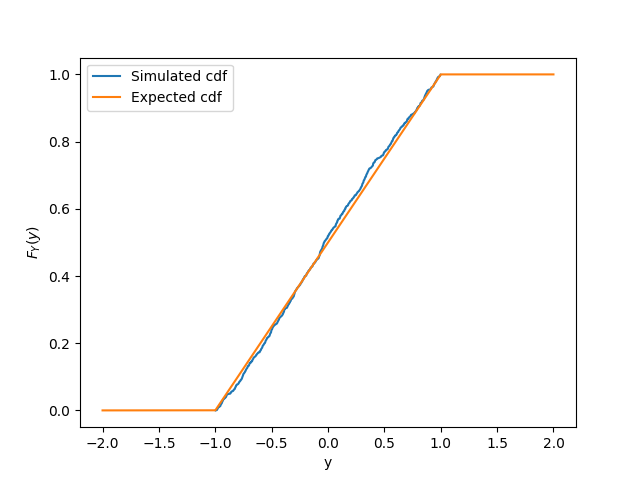
\includegraphics[width=100mm]{simulated_cdf.png}
    \caption{Simulated vs expected cdf plot of random variable Y}
    \label{cdf_plot}
\end{figure}
\end{frame}
\end{document}